\section{Understanding Recursion and Its Applications}
\subsection{What is Recursion?}

Recursion is a programming technique where a function calls itself in order to solve smaller instances of a problem. This is especially effective for problems that can be broken down into similar subproblems.

\subsubsection*{Key Components of Recursion}
\begin{itemize}
    \item \textbf{Base Case:} The stopping condition that ends the recursion. Without it, the function would call itself infinitely.
    \item \textbf{Recursive Case:} The part where the function calls itself with a modified parameter, bringing it closer to the base case.
\end{itemize}

\subsection{The Call Stack in Recursion}

When a function is called, it is added to the call stack, a data structure that keeps track of active function calls. Each recursive call pushes a new frame onto the stack. Once the base case is reached, the stack begins to unwind as each call returns its result.

\subsubsection*{Example: Call Stack for \texttt{factorial(4)}}

The factorial of a non-negative integer $n$ (denoted $n!$) is the product of all positive integers less than or equal to $n$.

\textbf{Recursive Definition}

\begin{itemize}
    \item \textbf{Base Case:} $factorial(0) = 1$
    \item \textbf{Recursive Case:} $factorial(n) = n \times factorial(n - 1)$
\end{itemize}

\begin{verbatim}
factorial(4)
→ 4 * factorial(3)
    → 3 * factorial(2)
        → 2 * factorial(1)
            → 1 * factorial(0)
                → 1 (base case)
\end{verbatim}
\begin{center}
    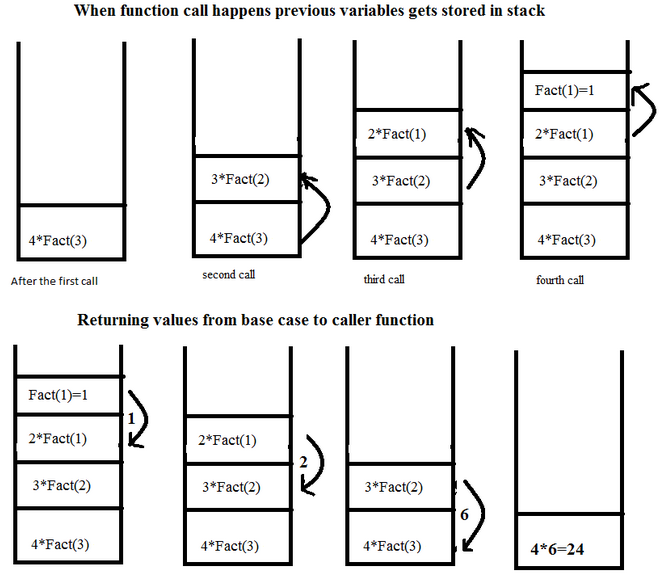
\includegraphics[width=5in]{../9. rBST/Notes/Assets/Call_Stack}
\end{center}

\section{Recursive Binary Search Trees (rBST): Contains, Insert, and Delete Operations}

\subsection{BST \texttt{contains()} Method}

The \texttt{contains()} method checks whether a given value exists in the BST.

\subsubsection*{Pseudocode}
\begin{verbatim}
def contains(value):
    if value == current_node.value:
        return True
    elif value < current_node.value and current_node.left:
        return contains(current_node.left, value)
    elif value > current_node.value and current_node.right:
        return contains(current_node.right, value)
    return False
\end{verbatim}

\subsubsection*{Example}

For a BST with root value 10:
\begin{verbatim}
    10
   /  \
  5   15
\end{verbatim}
Searching for 15:
\begin{verbatim}
→ 15 > 10 → move right
→ 15 == 15 → found
\end{verbatim}

\subsection{BST \texttt{insert()} Method}

The \texttt{insert()} method adds a value to the tree while maintaining the BST property.

\subsubsection*{Pseudocode}
\begin{verbatim}
def insert(value):
    if value < current_node.value:
        if current_node.left is None:
            current_node.left = new Node(value)
        else:
            insert(current_node.left, value)
    else:
        if current_node.right is None:
            current_node.right = new Node(value)
        else:
            insert(current_node.right, value)
\end{verbatim}

\subsubsection*{Example}
Inserting 7 into:
\begin{verbatim}
    10
   /  \
  5   15
\end{verbatim}
\begin{verbatim}
→ 7 < 10 → move left
→ 7 > 5 → insert to right of 5
\end{verbatim}

\subsection{BST \texttt{delete()} Method}

Deleting a node has three main cases:

\begin{enumerate}
    \item \textbf{Leaf Node (No Children):} Remove the node directly.
    \item \textbf{One Child:} Replace the node with its child.
    \item \textbf{Two Children:}
    \begin{itemize}
        \item Find the minimum value in the right subtree (in-order successor).
        \item Replace current node’s value with that minimum value.
        \item Recursively delete the in-order successor node.
    \end{itemize}
\end{enumerate}
\begin{center}
    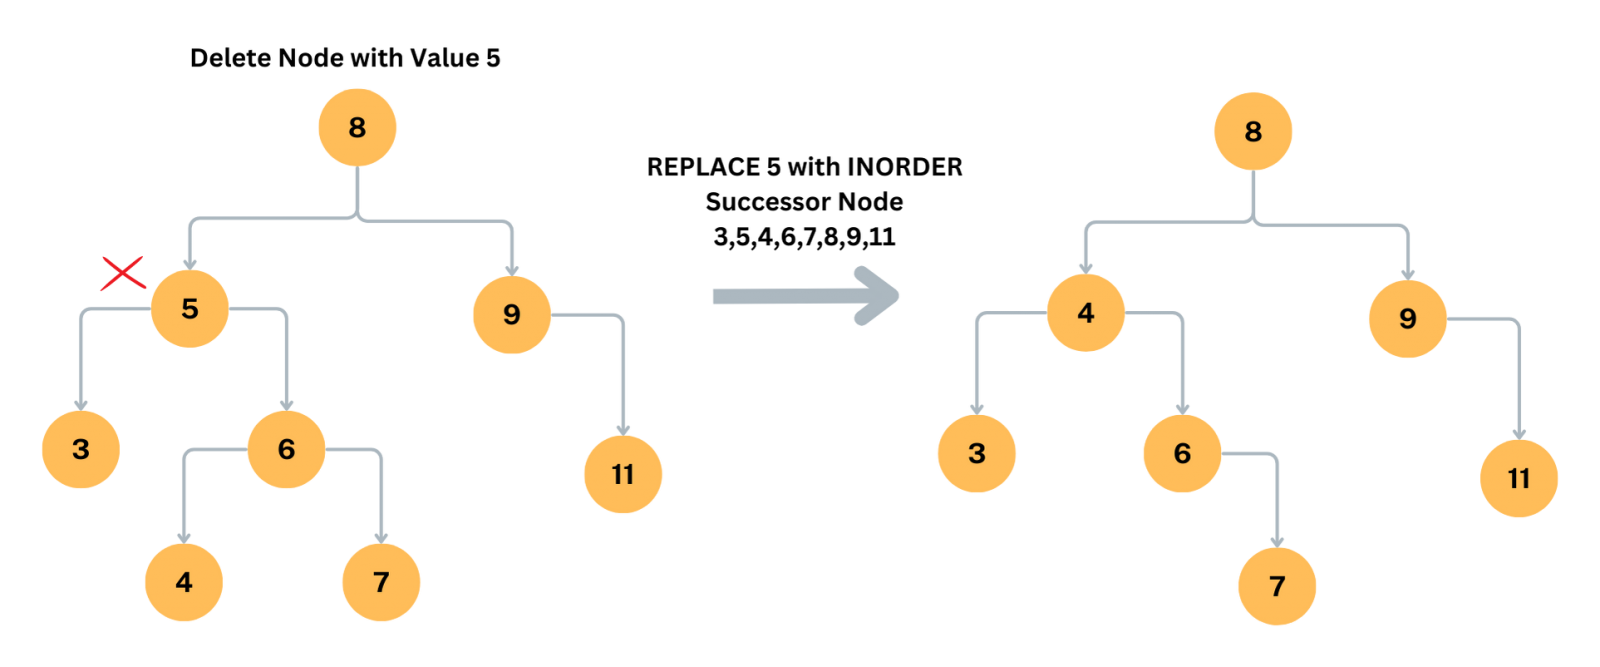
\includegraphics[width=5in]{../9. rBST/Notes/Assets/Node_Deletion_BST}    
\end{center}
\subsubsection*{Pseudocode}
\begin{verbatim}
def delete(value, current_node):
    if value < current_node.value:
        current_node.left = delete(value, current_node.left)
    elif value > current_node.value:
        current_node.right = delete(value, current_node.right)
    else:
        # Node with only one child or no child
        if current_node.left is None:
            return current_node.right
        elif current_node.right is None:
            return current_node.left
        # Node with two children
        temp = find_min(current_node.right)
        current_node.value = temp.value
        current_node.right = delete(temp.value, current_node.right)
    return current_node
\end{verbatim}

\subsubsection*{Finding Minimum}
\begin{verbatim}
def find_min(node):
    while node.left is not None:
        node = node.left
    return node
\end{verbatim}

\subsubsection*{Example}
Deleting node with value 21 (has two children):

\begin{verbatim}
         21
        /  \
      14    25
            /
          24
→ Minimum in right subtree: 24
→ Replace 21 with 24
→ Delete 24 from right subtree
\end{verbatim}

This preserves the BST structure while effectively removing the original node.
